\documentclass[]{article}
\usepackage{lmodern}
\usepackage{amssymb,amsmath}
\usepackage{ifxetex,ifluatex}
\usepackage{fixltx2e} % provides \textsubscript
\ifnum 0\ifxetex 1\fi\ifluatex 1\fi=0 % if pdftex
  \usepackage[T1]{fontenc}
  \usepackage[utf8]{inputenc}
\else % if luatex or xelatex
  \ifxetex
    \usepackage{mathspec}
  \else
    \usepackage{fontspec}
  \fi
  \defaultfontfeatures{Ligatures=TeX,Scale=MatchLowercase}
\fi
% use upquote if available, for straight quotes in verbatim environments
\IfFileExists{upquote.sty}{\usepackage{upquote}}{}
% use microtype if available
\IfFileExists{microtype.sty}{%
\usepackage{microtype}
\UseMicrotypeSet[protrusion]{basicmath} % disable protrusion for tt fonts
}{}
\usepackage[margin=1in]{geometry}
\usepackage{hyperref}
\hypersetup{unicode=true,
            pdftitle={Garden Experiment Power Analysis},
            pdfborder={0 0 0},
            breaklinks=true}
\urlstyle{same}  % don't use monospace font for urls
\usepackage{color}
\usepackage{fancyvrb}
\newcommand{\VerbBar}{|}
\newcommand{\VERB}{\Verb[commandchars=\\\{\}]}
\DefineVerbatimEnvironment{Highlighting}{Verbatim}{commandchars=\\\{\}}
% Add ',fontsize=\small' for more characters per line
\usepackage{framed}
\definecolor{shadecolor}{RGB}{248,248,248}
\newenvironment{Shaded}{\begin{snugshade}}{\end{snugshade}}
\newcommand{\KeywordTok}[1]{\textcolor[rgb]{0.13,0.29,0.53}{\textbf{#1}}}
\newcommand{\DataTypeTok}[1]{\textcolor[rgb]{0.13,0.29,0.53}{#1}}
\newcommand{\DecValTok}[1]{\textcolor[rgb]{0.00,0.00,0.81}{#1}}
\newcommand{\BaseNTok}[1]{\textcolor[rgb]{0.00,0.00,0.81}{#1}}
\newcommand{\FloatTok}[1]{\textcolor[rgb]{0.00,0.00,0.81}{#1}}
\newcommand{\ConstantTok}[1]{\textcolor[rgb]{0.00,0.00,0.00}{#1}}
\newcommand{\CharTok}[1]{\textcolor[rgb]{0.31,0.60,0.02}{#1}}
\newcommand{\SpecialCharTok}[1]{\textcolor[rgb]{0.00,0.00,0.00}{#1}}
\newcommand{\StringTok}[1]{\textcolor[rgb]{0.31,0.60,0.02}{#1}}
\newcommand{\VerbatimStringTok}[1]{\textcolor[rgb]{0.31,0.60,0.02}{#1}}
\newcommand{\SpecialStringTok}[1]{\textcolor[rgb]{0.31,0.60,0.02}{#1}}
\newcommand{\ImportTok}[1]{#1}
\newcommand{\CommentTok}[1]{\textcolor[rgb]{0.56,0.35,0.01}{\textit{#1}}}
\newcommand{\DocumentationTok}[1]{\textcolor[rgb]{0.56,0.35,0.01}{\textbf{\textit{#1}}}}
\newcommand{\AnnotationTok}[1]{\textcolor[rgb]{0.56,0.35,0.01}{\textbf{\textit{#1}}}}
\newcommand{\CommentVarTok}[1]{\textcolor[rgb]{0.56,0.35,0.01}{\textbf{\textit{#1}}}}
\newcommand{\OtherTok}[1]{\textcolor[rgb]{0.56,0.35,0.01}{#1}}
\newcommand{\FunctionTok}[1]{\textcolor[rgb]{0.00,0.00,0.00}{#1}}
\newcommand{\VariableTok}[1]{\textcolor[rgb]{0.00,0.00,0.00}{#1}}
\newcommand{\ControlFlowTok}[1]{\textcolor[rgb]{0.13,0.29,0.53}{\textbf{#1}}}
\newcommand{\OperatorTok}[1]{\textcolor[rgb]{0.81,0.36,0.00}{\textbf{#1}}}
\newcommand{\BuiltInTok}[1]{#1}
\newcommand{\ExtensionTok}[1]{#1}
\newcommand{\PreprocessorTok}[1]{\textcolor[rgb]{0.56,0.35,0.01}{\textit{#1}}}
\newcommand{\AttributeTok}[1]{\textcolor[rgb]{0.77,0.63,0.00}{#1}}
\newcommand{\RegionMarkerTok}[1]{#1}
\newcommand{\InformationTok}[1]{\textcolor[rgb]{0.56,0.35,0.01}{\textbf{\textit{#1}}}}
\newcommand{\WarningTok}[1]{\textcolor[rgb]{0.56,0.35,0.01}{\textbf{\textit{#1}}}}
\newcommand{\AlertTok}[1]{\textcolor[rgb]{0.94,0.16,0.16}{#1}}
\newcommand{\ErrorTok}[1]{\textcolor[rgb]{0.64,0.00,0.00}{\textbf{#1}}}
\newcommand{\NormalTok}[1]{#1}
\usepackage{graphicx,grffile}
\makeatletter
\def\maxwidth{\ifdim\Gin@nat@width>\linewidth\linewidth\else\Gin@nat@width\fi}
\def\maxheight{\ifdim\Gin@nat@height>\textheight\textheight\else\Gin@nat@height\fi}
\makeatother
% Scale images if necessary, so that they will not overflow the page
% margins by default, and it is still possible to overwrite the defaults
% using explicit options in \includegraphics[width, height, ...]{}
\setkeys{Gin}{width=\maxwidth,height=\maxheight,keepaspectratio}
\IfFileExists{parskip.sty}{%
\usepackage{parskip}
}{% else
\setlength{\parindent}{0pt}
\setlength{\parskip}{6pt plus 2pt minus 1pt}
}
\setlength{\emergencystretch}{3em}  % prevent overfull lines
\providecommand{\tightlist}{%
  \setlength{\itemsep}{0pt}\setlength{\parskip}{0pt}}
\setcounter{secnumdepth}{0}
% Redefines (sub)paragraphs to behave more like sections
\ifx\paragraph\undefined\else
\let\oldparagraph\paragraph
\renewcommand{\paragraph}[1]{\oldparagraph{#1}\mbox{}}
\fi
\ifx\subparagraph\undefined\else
\let\oldsubparagraph\subparagraph
\renewcommand{\subparagraph}[1]{\oldsubparagraph{#1}\mbox{}}
\fi

%%% Use protect on footnotes to avoid problems with footnotes in titles
\let\rmarkdownfootnote\footnote%
\def\footnote{\protect\rmarkdownfootnote}

%%% Change title format to be more compact
\usepackage{titling}

% Create subtitle command for use in maketitle
\providecommand{\subtitle}[1]{
  \posttitle{
    \begin{center}\large#1\end{center}
    }
}

\setlength{\droptitle}{-2em}

  \title{Garden Experiment Power Analysis}
    \pretitle{\vspace{\droptitle}\centering\huge}
  \posttitle{\par}
    \author{}
    \preauthor{}\postauthor{}
    \date{}
    \predate{}\postdate{}
  

\begin{document}
\maketitle

\section{Introduction}\label{introduction}

IN our study we focused on common plant community descriptors, which may
have significant consequences for the plant communities. Thes were above
ground biomass, species richness and abundance. For our experiment we
assumed simple one-way classification with one random effect. Therefore,
we are able to describe vales for a given descriptor under given
treatemnt in given block using the following formula:
\[\begin{matrix} \mathbb{E} [y_{ij}|a_j] = \mu + \beta_ix_{ij} + a_j + \varepsilon_{ij} \\ y_{ij}|a_j \sim indep.\ G\\ a_j \sim i.i.d.\ \mathcal{N}(0,\sigma_a^2) \end{matrix}\]
Where, \(y_{ij}\) represents community descriptor under treatement
\(i \in (1,..., 6)\), within block \(j \in (1,..., 6)\), and \(G\) is a
distribution for the \(y_{ij}|a_j\) with variance
\(\sigma^2_{\varepsilon}\).

In order to estimate power of our experimental setup (randomized
complete block design with six treatments and six control plots) we used
available estimates of the mean values, local and global variations in
biomass, species richness and abundance of plants in young successional
tropical forests.

First we look at the sample size (number of complete randomized blocks)
optimal for the detection of presumed ecologically significant shifts in
mean descriptor values. For the purposes of our exploratory analyses we
focused on considerably strong effects of approximately 20\% change of
the mean relative to the baseline values of our descriptors. Next, we
explored how different levels of variation between blocks and residual
variation affect power of our tests.

We performed Monte Carlo simulations, using the \emph{rsims} package ()
in R where hypothetical data was simulated and based on expected
\emph{random effect variation} (between block variation) \(\sigma_{a}\),
\emph{within block variation} or \emph{residual variance}
\(\sigma^2_{\varepsilon}\), and given effect size. Further we explored
also sensitivity of our power estimates on changing values of our
estimated parameters.

\section{Biomass}\label{biomass}

\subsection{Estimates of variation}\label{estimates-of-variation}

It is difficult to find estimates of variation in biomass for early
successional tropical forests. In one paper Sierra et al. (2007)
estimated a function of secondary forest biomass. Using their estimates
of the biomass as a function of the forest age:

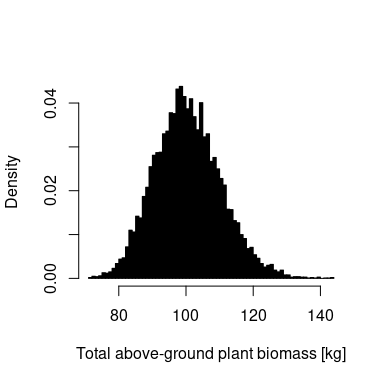
\includegraphics{garden_statistical_power_files/figure-latex/setup-1.pdf}

Unfortunately there are no estimates of variaiton for the functional
responce, however totoal aboveground biomass for secondary forests was
showed to be 46.4 \(\pm\) 4.3 T/ha (standard deviation) which gives for
our small plots an estimate of biomass around 116kg/ha indicating rather
low variabilitiy at least at the later stages of succession (what is the
age of this forest and what type of forest is this why is it relervant,
are there any closer estimates?). From the functional responce above we
expected to have approximately 95.7071619 kilograms of above ground
biomass. With probably higher variation. I estimated based on simple
proportional relationship that sd for early successional gardens might
be around (7 kg). To have standard deviation for a biomass equal to 7 we
numerically estimated the necessary variance for the normal
distribution. That turned out to be \(\sigma^2_{block} \sim\) 0.0054.

\includegraphics{garden_statistical_power_files/figure-latex/unnamed-chunk-1-1.pdf}
Fig. Histogram of final biomasses coming from a log-normal distribution
with expected standard deviation being \(\pm\) 7kg and expected mean
being around 95kg.

With these estimates we can now create a hypothetical dataset. Create a
dataset with six treatments within six experimental blocks.

\subsection{Randomization}\label{randomization}

Here we use our estimates to analyze power of our design to detect
decrease in plant biomass of about 5kg. This will depend on the
estimated between- and within-block variation.

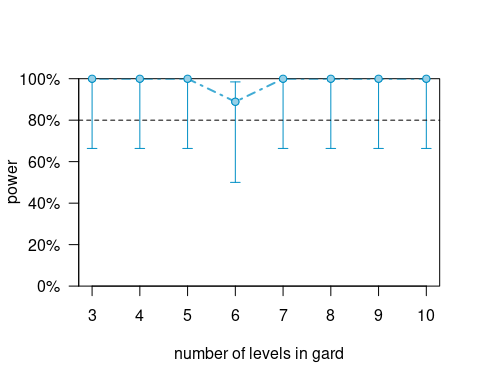
\includegraphics{garden_statistical_power_files/figure-latex/unnamed-chunk-3-1.pdf}

\begin{verbatim}
## Calculating power at 4 sample sizes along gard
\end{verbatim}

\begin{verbatim}
## Simulating: |                                                             |Simulating: |=                                                            |Simulating: |==                                                           |Simulating: |===                                                          |Simulating: |====                                                         |Simulating: |=====                                                        |Simulating: |======                                                       |Simulating: |=======                                                      |Simulating: |========                                                     |Simulating: |=========                                                    |Simulating: |==========                                                   |Simulating: |===========                                                  |Simulating: |============                                                 |Simulating: |=============                                                |Simulating: |==============                                               |Simulating: |===============                                              |Simulating: |================                                             |Simulating: |=================                                            |Simulating: |==================                                           |Simulating: |===================                                          |Simulating: |====================                                         |Simulating: |=====================                                        |Simulating: |======================                                       |Simulating: |=======================                                      |Simulating: |========================                                     |Simulating: |=========================                                    |Simulating: |==========================                                   |Simulating: |===========================                                  |Simulating: |============================                                 |Simulating: |=============================                                |Simulating: |==============================                               |Simulating: |===============================                              |Simulating: |================================                             |Simulating: |=================================                            |Simulating: |==================================                           |Simulating: |===================================                          |Simulating: |====================================                         |Simulating: |=====================================                        |Simulating: |======================================                       |Simulating: |=======================================                      |Simulating: |========================================                     |Simulating: |=========================================                    |Simulating: |==========================================                   |Simulating: |===========================================                  |Simulating: |============================================                 |Simulating: |=============================================                |Simulating: |==============================================               |Simulating: |===============================================              |Simulating: |================================================             |Simulating: |=================================================            |Simulating: |==================================================           |Simulating: |===================================================          |Simulating: |====================================================         |Simulating: |=====================================================        |Simulating: |======================================================       |Simulating: |=======================================================      |Simulating: |========================================================     |Simulating: |=========================================================    |Simulating: |==========================================================   |Simulating: |===========================================================  |Simulating: |============================================================ |Simulating: |=============================================================|(1/4) (1/4) Simulating: |                                                       |(1/4) Simulating: |=                                                      |(1/4) Simulating: |==                                                     |(1/4) Simulating: |===                                                    |
\end{verbatim}

\begin{verbatim}
## boundary (singular) fit: see ?isSingular
\end{verbatim}

\begin{verbatim}
## (1/4) Simulating: |====                                                   |(1/4) Simulating: |=====                                                  |(1/4) Simulating: |======                                                 |(1/4) Simulating: |=======                                                |(1/4) Simulating: |========                                               |
\end{verbatim}

\begin{verbatim}
## boundary (singular) fit: see ?isSingular
\end{verbatim}

\begin{verbatim}
## boundary (singular) fit: see ?isSingular
\end{verbatim}

\begin{verbatim}
## (1/4) Simulating: |=========                                              |(1/4) Simulating: |==========                                             |(1/4) Simulating: |===========                                            |
\end{verbatim}

\begin{verbatim}
## boundary (singular) fit: see ?isSingular
## boundary (singular) fit: see ?isSingular
\end{verbatim}

\begin{verbatim}
## (1/4) Simulating: |============                                           |
\end{verbatim}

\begin{verbatim}
## boundary (singular) fit: see ?isSingular
## boundary (singular) fit: see ?isSingular
\end{verbatim}

\begin{verbatim}
## (1/4) Simulating: |=============                                          |
\end{verbatim}

\begin{verbatim}
## boundary (singular) fit: see ?isSingular
\end{verbatim}

\begin{verbatim}
## (1/4) Simulating: |==============                                         |(1/4) Simulating: |===============                                        |
\end{verbatim}

\begin{verbatim}
## boundary (singular) fit: see ?isSingular
## boundary (singular) fit: see ?isSingular
\end{verbatim}

\begin{verbatim}
## (1/4) Simulating: |================                                       |(1/4) Simulating: |=================                                      |
\end{verbatim}

\begin{verbatim}
## boundary (singular) fit: see ?isSingular
\end{verbatim}

\begin{verbatim}
## (1/4) Simulating: |==================                                     |
\end{verbatim}

\begin{verbatim}
## boundary (singular) fit: see ?isSingular
## boundary (singular) fit: see ?isSingular
\end{verbatim}

\begin{verbatim}
## (1/4) Simulating: |===================                                    |(1/4) Simulating: |====================                                   |(1/4) Simulating: |=====================                                  |(1/4) Simulating: |======================                                 |
\end{verbatim}

\begin{verbatim}
## boundary (singular) fit: see ?isSingular
## boundary (singular) fit: see ?isSingular
\end{verbatim}

\begin{verbatim}
## (1/4) Simulating: |=======================                                |
\end{verbatim}

\begin{verbatim}
## boundary (singular) fit: see ?isSingular
## boundary (singular) fit: see ?isSingular
\end{verbatim}

\begin{verbatim}
## (1/4) Simulating: |========================                               |(1/4) Simulating: |=========================                              |(1/4) Simulating: |==========================                             |
\end{verbatim}

\begin{verbatim}
## boundary (singular) fit: see ?isSingular
\end{verbatim}

\begin{verbatim}
## (1/4) Simulating: |===========================                            |(1/4) Simulating: |============================                           |(1/4) Simulating: |=============================                          |(1/4) Simulating: |==============================                         |(1/4) Simulating: |===============================                        |
\end{verbatim}

\begin{verbatim}
## boundary (singular) fit: see ?isSingular
\end{verbatim}

\begin{verbatim}
## (1/4) Simulating: |================================                       |
\end{verbatim}

\begin{verbatim}
## boundary (singular) fit: see ?isSingular
## boundary (singular) fit: see ?isSingular
\end{verbatim}

\begin{verbatim}
## (1/4) Simulating: |=================================                      |(1/4) Simulating: |==================================                     |
\end{verbatim}

\begin{verbatim}
## boundary (singular) fit: see ?isSingular
\end{verbatim}

\begin{verbatim}
## (1/4) Simulating: |===================================                    |(1/4) Simulating: |====================================                   |(1/4) Simulating: |=====================================                  |(1/4) Simulating: |======================================                 |(1/4) Simulating: |=======================================                |(1/4) Simulating: |========================================               |
\end{verbatim}

\begin{verbatim}
## boundary (singular) fit: see ?isSingular
## boundary (singular) fit: see ?isSingular
\end{verbatim}

\begin{verbatim}
## (1/4) Simulating: |=========================================              |
\end{verbatim}

\begin{verbatim}
## boundary (singular) fit: see ?isSingular
\end{verbatim}

\begin{verbatim}
## (1/4) Simulating: |==========================================             |
\end{verbatim}

\begin{verbatim}
## boundary (singular) fit: see ?isSingular
## boundary (singular) fit: see ?isSingular
## boundary (singular) fit: see ?isSingular
\end{verbatim}

\begin{verbatim}
## (1/4) Simulating: |===========================================            |(1/4) Simulating: |============================================           |(1/4) Simulating: |=============================================          |(1/4) Simulating: |==============================================         |
\end{verbatim}

\begin{verbatim}
## boundary (singular) fit: see ?isSingular
## boundary (singular) fit: see ?isSingular
\end{verbatim}

\begin{verbatim}
## (1/4) Simulating: |===============================================        |
\end{verbatim}

\begin{verbatim}
## boundary (singular) fit: see ?isSingular
## boundary (singular) fit: see ?isSingular
\end{verbatim}

\begin{verbatim}
## (1/4) Simulating: |================================================       |(1/4) Simulating: |=================================================      |
\end{verbatim}

\begin{verbatim}
## boundary (singular) fit: see ?isSingular
## boundary (singular) fit: see ?isSingular
\end{verbatim}

\begin{verbatim}
## (1/4) Simulating: |==================================================     |(1/4) Simulating: |===================================================    |(1/4) Simulating: |====================================================   |(1/4) Simulating: |=====================================================  |
\end{verbatim}

\begin{verbatim}
## boundary (singular) fit: see ?isSingular
## boundary (singular) fit: see ?isSingular
\end{verbatim}

\begin{verbatim}
## (1/4) Simulating: |====================================================== |(1/4) Simulating: |=======================================================|(1/4) (2/4) (2/4) Simulating: |                                                       |(2/4) Simulating: |=                                                      |(2/4) Simulating: |==                                                     |(2/4) Simulating: |===                                                    |(2/4) Simulating: |====                                                   |(2/4) Simulating: |=====                                                  |(2/4) Simulating: |======                                                 |(2/4) Simulating: |=======                                                |(2/4) Simulating: |========                                               |(2/4) Simulating: |=========                                              |(2/4) Simulating: |==========                                             |(2/4) Simulating: |===========                                            |(2/4) Simulating: |============                                           |(2/4) Simulating: |=============                                          |
\end{verbatim}

\begin{verbatim}
## boundary (singular) fit: see ?isSingular
\end{verbatim}

\begin{verbatim}
## (2/4) Simulating: |==============                                         |(2/4) Simulating: |===============                                        |(2/4) Simulating: |================                                       |(2/4) Simulating: |=================                                      |(2/4) Simulating: |==================                                     |(2/4) Simulating: |===================                                    |(2/4) Simulating: |====================                                   |(2/4) Simulating: |=====================                                  |(2/4) Simulating: |======================                                 |(2/4) Simulating: |=======================                                |(2/4) Simulating: |========================                               |(2/4) Simulating: |=========================                              |(2/4) Simulating: |==========================                             |(2/4) Simulating: |===========================                            |(2/4) Simulating: |============================                           |(2/4) Simulating: |=============================                          |(2/4) Simulating: |==============================                         |(2/4) Simulating: |===============================                        |(2/4) Simulating: |================================                       |
\end{verbatim}

\begin{verbatim}
## boundary (singular) fit: see ?isSingular
\end{verbatim}

\begin{verbatim}
## (2/4) Simulating: |=================================                      |(2/4) Simulating: |==================================                     |(2/4) Simulating: |===================================                    |(2/4) Simulating: |====================================                   |(2/4) Simulating: |=====================================                  |(2/4) Simulating: |======================================                 |(2/4) Simulating: |=======================================                |(2/4) Simulating: |========================================               |(2/4) Simulating: |=========================================              |(2/4) Simulating: |==========================================             |(2/4) Simulating: |===========================================            |(2/4) Simulating: |============================================           |(2/4) Simulating: |=============================================          |(2/4) Simulating: |==============================================         |(2/4) Simulating: |===============================================        |(2/4) Simulating: |================================================       |(2/4) Simulating: |=================================================      |(2/4) Simulating: |==================================================     |(2/4) Simulating: |===================================================    |(2/4) Simulating: |====================================================   |(2/4) Simulating: |=====================================================  |(2/4) Simulating: |====================================================== |(2/4) Simulating: |=======================================================|(2/4) (3/4) (3/4) Simulating: |                                                       |(3/4) Simulating: |=                                                      |(3/4) Simulating: |==                                                     |(3/4) Simulating: |===                                                    |(3/4) Simulating: |====                                                   |(3/4) Simulating: |=====                                                  |(3/4) Simulating: |======                                                 |(3/4) Simulating: |=======                                                |(3/4) Simulating: |========                                               |(3/4) Simulating: |=========                                              |(3/4) Simulating: |==========                                             |(3/4) Simulating: |===========                                            |(3/4) Simulating: |============                                           |(3/4) Simulating: |=============                                          |(3/4) Simulating: |==============                                         |(3/4) Simulating: |===============                                        |(3/4) Simulating: |================                                       |(3/4) Simulating: |=================                                      |(3/4) Simulating: |==================                                     |(3/4) Simulating: |===================                                    |(3/4) Simulating: |====================                                   |(3/4) Simulating: |=====================                                  |(3/4) Simulating: |======================                                 |(3/4) Simulating: |=======================                                |(3/4) Simulating: |========================                               |(3/4) Simulating: |=========================                              |(3/4) Simulating: |==========================                             |(3/4) Simulating: |===========================                            |(3/4) Simulating: |============================                           |(3/4) Simulating: |=============================                          |(3/4) Simulating: |==============================                         |(3/4) Simulating: |===============================                        |(3/4) Simulating: |================================                       |(3/4) Simulating: |=================================                      |(3/4) Simulating: |==================================                     |(3/4) Simulating: |===================================                    |(3/4) Simulating: |====================================                   |(3/4) Simulating: |=====================================                  |(3/4) Simulating: |======================================                 |(3/4) Simulating: |=======================================                |(3/4) Simulating: |========================================               |(3/4) Simulating: |=========================================              |(3/4) Simulating: |==========================================             |(3/4) Simulating: |===========================================            |(3/4) Simulating: |============================================           |(3/4) Simulating: |=============================================          |(3/4) Simulating: |==============================================         |(3/4) Simulating: |===============================================        |(3/4) Simulating: |================================================       |(3/4) Simulating: |=================================================      |(3/4) Simulating: |==================================================     |(3/4) Simulating: |===================================================    |(3/4) Simulating: |====================================================   |(3/4) Simulating: |=====================================================  |(3/4) Simulating: |====================================================== |(3/4) Simulating: |=======================================================|(3/4) (4/4) (4/4) Simulating: |                                                       |(4/4) Simulating: |=                                                      |(4/4) Simulating: |==                                                     |(4/4) Simulating: |===                                                    |(4/4) Simulating: |====                                                   |(4/4) Simulating: |=====                                                  |(4/4) Simulating: |======                                                 |(4/4) Simulating: |=======                                                |(4/4) Simulating: |========                                               |(4/4) Simulating: |=========                                              |(4/4) Simulating: |==========                                             |(4/4) Simulating: |===========                                            |(4/4) Simulating: |============                                           |(4/4) Simulating: |=============                                          |(4/4) Simulating: |==============                                         |(4/4) Simulating: |===============                                        |(4/4) Simulating: |================                                       |(4/4) Simulating: |=================                                      |(4/4) Simulating: |==================                                     |(4/4) Simulating: |===================                                    |(4/4) Simulating: |====================                                   |(4/4) Simulating: |=====================                                  |(4/4) Simulating: |======================                                 |(4/4) Simulating: |=======================                                |(4/4) Simulating: |========================                               |(4/4) Simulating: |=========================                              |(4/4) Simulating: |==========================                             |(4/4) Simulating: |===========================                            |(4/4) Simulating: |============================                           |(4/4) Simulating: |=============================                          |(4/4) Simulating: |==============================                         |(4/4) Simulating: |===============================                        |(4/4) Simulating: |================================                       |(4/4) Simulating: |=================================                      |(4/4) Simulating: |==================================                     |(4/4) Simulating: |===================================                    |(4/4) Simulating: |====================================                   |(4/4) Simulating: |=====================================                  |(4/4) Simulating: |======================================                 |
\end{verbatim}

\begin{verbatim}
## boundary (singular) fit: see ?isSingular
\end{verbatim}

\begin{verbatim}
## (4/4) Simulating: |=======================================                |(4/4) Simulating: |========================================               |(4/4) Simulating: |=========================================              |(4/4) Simulating: |==========================================             |(4/4) Simulating: |===========================================            |(4/4) Simulating: |============================================           |(4/4) Simulating: |=============================================          |(4/4) Simulating: |==============================================         |(4/4) Simulating: |===============================================        |(4/4) Simulating: |================================================       |(4/4) Simulating: |=================================================      |(4/4) Simulating: |==================================================     |(4/4) Simulating: |===================================================    |(4/4) Simulating: |====================================================   |(4/4) Simulating: |=====================================================  |(4/4) Simulating: |====================================================== |(4/4) Simulating: |=======================================================|(4/4) 
\end{verbatim}

\includegraphics{garden_statistical_power_files/figure-latex/unnamed-chunk-3-2.pdf}

Here we show an example dataset generated using log-normal mean 95,
between-block standard deviation \(\sqrt{\sigma_{block}} =\) 7.01,
within-block standard deviation \(\sqrt{\sigma_{error}}=\) 7.01 and
effect size of -10 kg.

\includegraphics{garden_statistical_power_files/figure-latex/unnamed-chunk-4-1.pdf}
Fig . Simulated 99 datasets with 6 treatments grouped within six blocks
and a hypothetical effect size of high herbivory (h2) to be -10.

With the above assumptions we were able to obtain the power of 0.68
\(\pm\) 0.09 (95\% bootstraped CI). Which is within acceptable level of
statistical power.

\section{Species richness and woody plant
abundance}\label{species-richness-and-woody-plant-abundance}

\subsection{Estimates of variation}\label{estimates-of-variation-1}

We expected to find approximately 30 \(\pm\) 5 plant species (herbaceous
and woody plants) per plot (Leps, personal communication). It is
difficult to estimates for the abundance of stems having DBH greater of
equal to 1cm. However, Based on Whitfeld et al. (2012) and our own
experience we expected to have (similarily to the number of species)
approximately 30 \(\pm\) 5 stems per 25m\(^2\) experimental plot.

\subsection{Randomization}\label{randomization-1}

As above we create random dataset for for number of species and
abundance of stems \(\leq\) 1 cm DBH, and estimate the expected power of
our design.

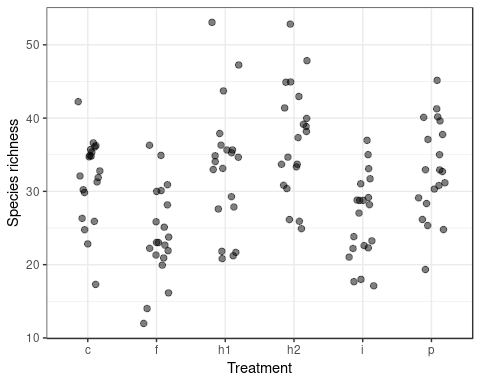
\includegraphics{garden_statistical_power_files/figure-latex/unnamed-chunk-5-1.pdf}

Fig X. \ldots{}

\section{Sample size, within-block and between-block
variation}\label{sample-size-within-block-and-between-block-variation}

Here we want do analyze sensitivity of our estimates on the expected
power of our analyses. We perform a randomization manipulating three
parameters: number of samples, between block variation and within block
noise (within block variation)

\begin{Shaded}
\begin{Highlighting}[]
\CommentTok{# mcrands <- 999}
\CommentTok{# wbsd <- round(sqrt(seq(0.0005, 0.01, by = 0.0025)),3)}
\CommentTok{# bbsd <- round(sqrt(seq(0.0005, 0.01, by = 0.0025)),3)}
\CommentTok{# ssize <- seq(5, 20, by=1)#sample size}
\CommentTok{# # leff_size varry the effect size? }
\CommentTok{# # Random effect standard deviation}
\CommentTok{# resmatgard1 <- matrix(0, }
\CommentTok{#                       nrow = length(wbsd),}
\CommentTok{#                       ncol = length(ssize))}
\CommentTok{# rownames(resmatgard1) <- as.character(round(wbsd, 3))}
\CommentTok{# colnames(resmatgard1) <- ssize}
\CommentTok{# }
\CommentTok{# for(row in wbsd)\{}
\CommentTok{#   for(col in ssize)\{}
\CommentTok{#     temp_res <- randDat(rands=mcrands,}
\CommentTok{#                     pattern=c(1,0,0,leff_size,0,0),}
\CommentTok{#                     mu=log(mu),}
\CommentTok{#                     sdg = row,}
\CommentTok{#                     sd = sd,}
\CommentTok{#                     ngard = col,}
\CommentTok{#                     nplot = 6)}
\CommentTok{#     rd <- temp_res$fits}
\CommentTok{#     p_hat <- sum(rd/mcrands)}
\CommentTok{#     }
\CommentTok{#     resmatgard1[as.character(row),as.character(col)] <- p_hat}
\CommentTok{#     }
\CommentTok{#   \}}
\CommentTok{# \}}
\CommentTok{# }
\CommentTok{# levelplot(resmatgard1, xlab = "Between block variation",}
\CommentTok{#           ylab = "Number of blocks") +}
\CommentTok{#   as.layer(contourplot(resmatgard1, col = "red"))}
\CommentTok{# }
\CommentTok{# }
\CommentTok{# # With simr}
\CommentTok{# vars <- seq(0.003, 0.090, by=0.015)}
\CommentTok{# resmatgard1 <- matrix(0, }
\CommentTok{#                       nrow = length(vars),}
\CommentTok{#                       ncol = length(vars))}
\CommentTok{# rownames(resmatgard1) <- as.character(round(vars, 3))}
\CommentTok{# colnames(resmatgard1) <- as.character(round(vars, 3))}
\CommentTok{# }
\CommentTok{# mcrands <- 99}
\CommentTok{# counter <- 1}
\CommentTok{# dims    <- length(vars)}
\CommentTok{# for (i in vars)\{}
\CommentTok{#   for(j in vars)\{}
\CommentTok{#     counter <- counter + 1}
\CommentTok{#     print(counter/(dims*dims))}
\CommentTok{#     VarCorr(bio_rbl) <- i  #}
\CommentTok{#     sigma(bio_rbl) <- sqrt(j)}
\CommentTok{#     est <- powerSim(bio_rbl, nsim = mcrands)}
\CommentTok{#     resmatgard1[as.character(i),}
\CommentTok{#                 as.character(j)] <- summary(est)$mean}
\CommentTok{#   \}}
\CommentTok{# \}}
\CommentTok{# }
\CommentTok{# levelplot(resmatgard1, ylab = "Sigma",}
\CommentTok{#           xlab = "VarCorr")}
\end{Highlighting}
\end{Shaded}


\end{document}
